\documentclass{article}

% if you need to pass options to natbib, use, e.g.:
%     \PassOptionsToPackage{numbers, compress}{natbib}
% before loading neurips_2020

\usepackage{natbib}
\bibliographystyle{abbrvnat}
\setcitestyle{authoryear,open={(},close={)}}

% commands for comments
\usepackage[dvipsnames]{xcolor}
\newcommand{\todo}[1]{\textbf{\textcolor{Red}{(TODO: #1)}}}

% ready for submission
%\usepackage{neurips_2020}

% to compile a preprint version, e.g., for submission to arXiv, add add the
% [preprint] option:
    \usepackage[preprint]{neurips_2020}

% to compile a camera-ready version, add the [final] option, e.g.:
%  \usepackage[final]{neurips_2020}

% to avoid loading the natbib package, add option nonatbib:
%     \usepackage[nonatbib]{neurips_2020}

\usepackage[utf8]{inputenc} % allow utf-8 input
\usepackage[T1]{fontenc}    % use 8-bit T1 fonts
\usepackage[colorlinks,citecolor=blue]{hyperref}       % hyperlinks
\usepackage{url}            % simple URL typesetting
\usepackage{booktabs}       % professional-quality tables
\usepackage{amsfonts}       % blackboard math symbols
\usepackage{nicefrac}       % compact symbols for 1/2, etc.
\usepackage{microtype}      % microtypography
\usepackage{amsmath}
\usepackage{graphicx}		% include figures
\usepackage{float}			% keeps figures in place
\usepackage{xurl}           % keeps URL from overflowing

\title{Joint Multimodal Embeddings}

% The \author macro works with any number of authors. There are two commands
% used to separate the names and addresses of multiple authors: \And and \AND.
%
% Using \And between authors leaves it to LaTeX to determine where to break the
% lines. Using \AND forces a line break at that point. So, if LaTeX puts 3 of 4
% authors names on the first line, and the last on the second line, try using
% \AND instead of \And before the third author name.

\author{%
   Patrick Kahardipraja%\thanks{Use footnote for providing further information
    %about author (webpage, alternative address)---\emph{not} for acknowledging
    %funding agencies.} \\
  %Department of Computer Science\\
  %Cranberry-Lemon University\\
  %Pittsburgh, PA 15213 \\
  %\texttt{hippo@cs.cranberry-lemon.edu} \\
  % examples of more authors
  \And
   Laura Kopf \\
  % Affiliation \\
  % Address \\
  % \texttt{email} \\
  % \AND
  % Coauthor \\
  % Affiliation \\
  % Address \\
  % \texttt{email} \\
  % \And
  % Coauthor \\
  % Affiliation \\
  % Address \\
  % \texttt{email} \\
  % \And
  % Coauthor \\
  % Affiliation \\
  % Address \\
  % \texttt{email} \\
}

\begin{document}

\maketitle

\begin{abstract}
Multimodal vision and language tasks such as visual question answering (VQA) are challenging, because they require both the understanding of image content and natural language. To solve multimodal problems it is crucial to represent data in a meaningful way. One way to do this/common approach is to project joint representations to the same space using all of the modalities as input to establish inter-modal relationships. In this project we will investigate whether joint representations derived from pre-trained models are better compared to the joint representations learned from a task-specific model. In an effort to answer this question, we will compare the pre-trained and multi-task Vision-and-Language BERT (ViLBERT) \citep{lu2019vilbert, lu2020multitask} models to the task-specific deep Modular Co-Attention Network (MCAN) \citep{yu2019mcan} on a VQA task and evaluate grounding. Our experimental results demonstrate that \todo{give short summary of our results}. Our code is (publicly) available at \url{https://github.com/lkopf/joint-multimodal-embeddings}.
\end{abstract}

\section{Introduction}

In recent years there have been significant advancements in several language and vision tasks such as image-text retrieval \citep{wang2016retrieval}, visual commonsense reasoning \citep{zellers2019vcr}, visual entailment \citep{xie2019entailment} and visual question answering \citep{antol2015vqa, malinowski2014vqa, ban, zhao2018vqa}. In its most common form, the VQA task requires an algorithm to provide the correct answer for a natural language question asked about an input image. Solving the VQA task stands out as particularly challenging, because it also involves solving many subtasks like object detection, activity recognition, knowledge base reasoning, and commonsense reasoning. 

\todo{find better transition}
A variety of models have been developed to solve this task, using different methods such as stacked attention networks \citep{yang2016vqa}, bottom-up and top-down attention mechanism \citep{Anderson_2018_CVPR}, and compositional attention networks \citep{hudson2018mac} to name a few. In our project we will compare two attention-based models that have different approaches to solving the VQA problem: MCAN and ViLBERT.

MCAN consists of Modular Co-Attention (MCA) layers cascaded in depth. Each layer is composed of two basic attention units, self-attention of questions and images, as well as the guided-attention of images. The input question is transformed into GloVe word embeddings and subsequently passed through a one layer LSTM network. In the multimodal fusion textual and image representations are jointly embedded into the same space and fed into a classifier which predicts the final answer.

ViLBERT is fairly similar to the MCAN architecture, but in contrast is not task specific. In our project we will refer to two ViLBERT models. The first being the ViLBERT model pretrained on the Conceptual Captions dataset originally proposed by \cite{lu2019vilbert}, and the second one being the multi-task ViLBERT model recently introduced by \cite{lu2020multitask}. ViLBERT is a pre-trained model that is extending the BERT language model to jointly represent images and text. It processes visual and textual inputs in separate streams that interact through co-attentional transformer layers. The pre-trained model is then put to four vision-and-language tasks: visual question answering, visual commonsense reasoning, referring expressions, and caption-based image retrieval. Multi-task ViLBERT has a similar architecture, but it is trained jointly on 12 datasets on the same four categories of tasks as previously mentioned. \cite{lu2020multitask} argue that joint training can improve the performance compared to single-task training with the same architecture. \todo{add specific reason why we also include multi-task ViLBERT}

In comparison to MCAN, only one modality can be used to guide another modality while ViLBERT allows both modalities to exchange information simultaneously. Another difference lies in the fusing method the architectures use. MCAN learns to project textual and image representations to a shared space, while ViLBERT applies an element-wise product between visual and linguistic representations.

It still remains unclear to which extent the models that solve the VQA task understood the visual-language concepts. \cite{agrawal12018gvqa} argue that VQA models are heavily driven by superficial correlations in the training data and lack sufficient image grounding. To gain an insight into what the models are learning, we focus on whether the models are able to ground questions accurately. The GQA dataset \citep{hudson2019gqa} seeks to address the shortcomings of previous VQA datasets and also includes a metric to evaluate grounding.

Our project aims to examine the question whether representations derived from pre-trained models such es ViLBERT are actually better compared to representations learned from a task-specific model such as MCAN. In order to better understand the characteristics of the more successful network architecture we apply both to a VQA task. We build our experimental setup on two pre-existing models and will conduct two modifications to the MCAN. One method will be to replace GloVe as embedding with BERT, and the second method will be to replace the LSTM question encoder with a BERT encoder. We finetune both methods and analyze how this affects the model’s performance. We train and evaluate the modified MCAN architectures on the benchmark VQA-v2 dataset \citep{goyal2017vqa2} and and compare it to the results of both to the results of the original MCAN architecture and ViLBERT. In order to evaluate grounding we will evaluate the MCAN architectures on GQA and compare these results to ViLBERT based on multi-task learning on GQA \citep{lu2020multitask}. \todo{Give short preview of our results. Add missing steps in our experimantal setup/evaluation method}
\todo{General note: revise Introduction according to our report: add/shorten paragraphs where needed}

\section{Related Work}

mcan\citep{yu2019mcan}

vilbert\citeauthor{lu2019vilbert}

\subsection{Advances in Multimodal Embeddings} \label{embeds}
%bilinear?

\subsection{Grounding}

\subsection{Visual Question Answering}

%this paragraph is probably too long. Maybe focus more on VQA or make the connectio to the other tasks more obvious.
The integration of vision and language tasks has significantly advanced multi-disciplinary research/work from fields of computer vision, natural language processing and deep learning. The underlying challenge of this integration is to find methods that understand visual or textual content and are able to generate visual or textual content according to the given task. To solve these challenges multimodal learning models are created that can process and relate information from multiple modalities such as linguistic and visual information. The range of different language and vision integration tasks is quite broad, which is why will only name a few to give a (short) overview. Visual description generation aims to generate a textual description given a visual input \citep{plummer2015vdg} Visual referring expression goes in two directions and includes the task of referring expression generation and comprehension. The former generates a referring expression for a given target object present in a visual scene \citep{fitzgerald2013learning}. Given an image and referring expression, comprehension is performed by localizing an object in an image by using bounding boxes \citep{nagaraja2016modeling}. There are also approaches that combine both generation and comprehension \citep{yu2016modeling} Visual question answering answers questions about visual information \citep{antol2015vqa}. Visual reasoning aims to go beyond the VQA benchmark and answer sophisticated queries by reasoning about visual input \citep{johnson2017clevr}.

In our project we will mainly focus on the visual question answering task. VQA is a  multi-modal challenging task and intersects with the previously mentioned tasks. The goal of VQA is to learn a model to produce a natural language answer about free-form, open-ended natural language questions by reasoning about presented visual content. The visual input can be either images or videos. Furthermore we will only focus on images in the further discussion. In regards to VQA demanding multi-modal knowledge beyond a single domain, it has been widely accepted as an AI-complete task. \cite{geman2015visual} have considered VQA as the Visual Turing Test, where human-level abilities to semantically understanding visual information and answering questions are expected. Solving the VQA task efficiently can result in various potential applications. It can help blind users communicate with pictures, allow users of online educational services to interact with images, summarize visual data for surveillance data analysis and lastly through image retrieval improve the search queries on online shopping sites \citep{manmadhan2020vqa}.

\begin{figure}[H]
	\centering
	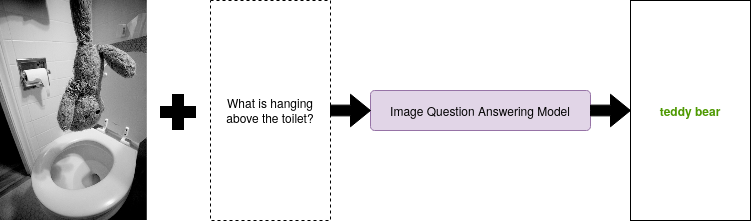
\includegraphics[width=\linewidth]{vqa_teddy_tiny.png}
	\caption{Given an image and question as input, the visual question answering model predicts an answer to it.}
	\label{fig:vqa-graph}
\end{figure}

Compared to other vision and language tasks such as visual description generation, visual referring expression, VQA stands out as a particularly challenging task for various reasons. In order to predict an accurate answer, the VQA model requires a fine-grained semantic understanding of both the image and the question. Acquiring this involves solving a wide range of computer vision sub tasks such as object recognition, object detection, attribute classification, scene classification, counting, activity recognition, spatial relationships among objects, commonsense reasoning and knowledge-base reasoning \citep{manmadhan2020vqa}. Unlike to other tasks, where the question to be answered is fixed and only the image changes, the questions in VQA are not predetermined. Another challenge is the high-dimensionality of the supporting visual information.

Within the last couple years many researchers have proposed different solutions for the VQA task that generally follow the same structure. The general VQA algorithm can be divided up into three phases: Firstly image featurization and question featurization, secondly joint comprehension, and lastly answer generation.
In the first phase the given image and question are processed independently to obtain separate vector representations. There are multiple ways to extract information about images and questions of which we will only present a selected few.

In the process of image featurization the system/model needs to extract relevant features of the image to understand the image content. The image feature describes an image as a numerical vector, in order for it to be applied to different mathematical operations. Most VQA models use pre-trained deep neural network models for image featurization, of which convolutional neural network (CNN) \citep{krizhevsky2012imagenet} pre-trained on ImageNet \citep{russakovsky2015imagenet} is the most widely used one because of its good performance. The predominant CNN models trained on ImageNet include AlexNet \citep{krizhevsky2012imagenet}, ZFNet \citep{zeiler2014visual}, VGGNet \citep{simonyan2015very}, GoogleNet \citep{szegedy2015going} and lastly ResNet \citep{residual}, which is currently the most used one by researchers.

Plain text or strings cannot be processed by most machine learning algorithms and almost all deep learning architectures. This demands questions to be prepared in a way that can be processed by the system/model. Word embeddings enable the necessary preprocessing for question featurization. Embeddings can be defined as numerical vectors that represent words or phrases from a vocabulary. These vectors represent a collection of features that hold information about the relation between words. Since word embeddings are trained on word co-occurence, they capture semantic, morphological or contextual information. Different training algorithms and text corpora have an influence on the generated word embeddings. This makes it a challenging task to choose the best embedding for the VQA task.

% find reference for one-hot vector
Early embedding models have been count based models such as one-hot vector and co-occurence matrix \citep{miller1991contextual}. They are simple to implement and interpret, but quickly run into issues concerning their fast growth as the length of the sparse vector is generally the size of the vocabulary. An alternative method for representing a word is to use a short and dense vector. Prediction based models such as CBOW and skip-gram (also called word2vec) \citep{mikolov2013efficient} directly learn word representation and use neural network as their basic component to train a classifier on a binary prediction task. In the last few years hybrid models that combine count based and predict based methods to produce a word embedding have become more popular in NLP research. One prominent example are global vectors (GloVe) \citep{pennington2014glove}, which perform more accurate than skip-gram, because the global corpus statistics are captured directly by the model. An even newer form of embeddings are contextualized word representations such as ELMo \citep{peters2018elmo} and BERT \citep{devlin-etal-2019-bert}.

\begin{figure}[H]
	\centering
	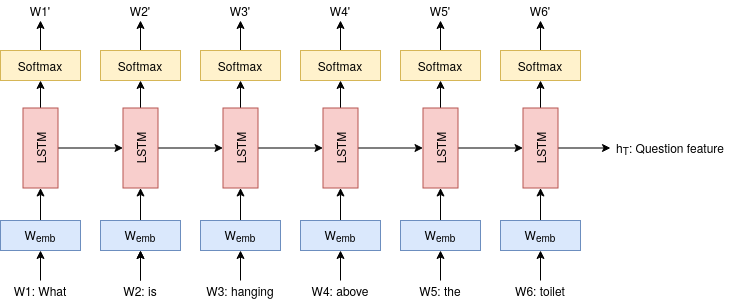
\includegraphics[width=\linewidth]{lstm.png}
	\caption{Basic architecture of LSTM question feature extraction.}
	\label{fig:lstm}
\end{figure}

In advanced methods for question feature extraction in VQA neural networks such as convolutional neural network \citep{krizhevsky2012imagenet}, long short term memory (LSTM) \citep{lstm} and gated recurrent unit (GRU) \citep{cho2014gru} are used. The latter two belong to the recurrent neural network (RNN) family \citep{elman1990finding} \cite{young2018recent} state that sequence based models like RNN do better than word sequence independent methods like word2vec and also claim that LSTM are generally preferred by VQA researchers. It should also be noted that RNN models are not used independently, but are always combined with any traditional embeddings (mentioned previously) that are fed as input to LSTM or GRU. Figure \ref{fig:lstm} shows the basic architecture of LSTM where word embeddings are the input and question feature is generated as output. Both LSTM and GRU are gating based architectures that are designed to capture long-range dependencies and solve the vanishing gradient problem. The LSTM layer has memory cells where it can store context information e.g. of words in a sequence, when the input is a question. The memory is controlled by gates, of which one gate at each input state decides how much of the new input should be written to the memory cell, and how much of the current content of the memory cell should be forgotten. In Figure \ref{fig:lstm} $h_T$ represents the output state vector from the last time step that is used as a question feature. GRU is an alternative to the LSTM, which has fewer gates and does not have separate memory cells.

After the image features and question features are extracted, the features are mapped to a joint space and then combined to generate an answer to the question about an image. There is a wide range of techniques for joint comprehension of image and text of which some were already discussed in section \ref{embeds}. We will present a selection methods for combining multi-modal features that is particularly relevant for the VQA task.

\todo{First write section ‘Advances in Multimodal Embeddings’ and then select relevant methods for VQA. Possible inclusions could be: baseline models, encoder-decoder architecture, joint attention models. Briefly describe the architecture, then discuss advantages/disadvantages}

There are numerous publically available datasets for validating VQA models with their own focus. \todo{depending on how long this section gets just briefly mention some datasets and refer to the discussion of VQA 2.0 in section 4.1. Also include critique of datasets}
The most used evaluation metric for state-of-the-art VQA models is accuracy, which represents the ratio of the number of correctly answered questions to the number of total questions. 

\subsection{Modular Co-Attention Network (MCAN)}
% explain SA & GA, MCA
%inter-modal, intra-modal and dense interaction modeling
% inspiration of co-attention?
In VQA, extracting discriminative features for textual and image representations are important in order to obtain fine-grained semantic understanding of both the image and the question. However, using global features extracted from the whole image to represent visual information may introduce noisy information that are irrelevant to the question (e.g. the case where only a small region of the image that relates to a question). On the other side, natural language questions may also contain words that are not relevant to the image and therefore can be also considered as noise. This leads to co-attention learning approach to jointly learn the attentions for both the image and the question simultaneously, which allows the model to extract more discriminative visual and textual representations. 

Several methods have been proposed for co-attention learning in VQA. \citet{yu2018beyond} separated the co-attention method into two steps, self-attention for question attention and visual attention conditioned on attended question representation. In their approach, multiple attention maps can also be used to improve the capacity of the attended visual representation, where it is fused at a later stage with the attended question representation through multi-modal factorized high-order pooling (MFH). \citet{Nguyen_2018_CVPR} proposed dense co-attention network (DCN) which establish bi-directional interactions between textual and visual modalities by generating attention map on question words for each image region and vice versa. \citet{ban} introduced bilinear attention networks (BAN), where bilinear attention map is used to reduce the computational cost to learn attention distribution for every pair of question words and image regions. They also used low-rank bilinear pooling to produce joint question and image representation. However MFH lacks dense interaction modeling between questions and images. DCN and BAN also do not model intra-modal attention.

To address the aforementioned problems, \citet{yu2019mcan} proposed modular co-attention network (MCAN), which simultaneously models dense intra- and inter- modal interactions. MCAN is composed of stacked modular co-attention (MCA) layer which consists of the self-attention (SA) and the guided-attention (GA) unit based on scaled dot-product attention \citep{transformers}. The SA unit consists of multi-head attention layer and feed-forward neural network (FFNN) layer. It accepts group of input features $X = [x_{1}, \dots, x_{m}]$ where $m$ is number of features and pass it through the multi-head attention module to learn pairwise relationship between every possible pairing $\langle x_{i},x_{j} \rangle$ in $X$ to obtain attended output features $Z$ using weighted summation of $X$. The output of the multi-head attention layer $Z$ is then feeded through two fully-connected layers with ReLU activation \citep{relu} and dropout units \citep{dropout}. A residual connection \citep{residual} is employed around each of the two layers, followed by layer normalization \citep{ba2016layer} to improve optimization.

The GA unit is almost similar to the SA unit. It is composed of multi-head attention and FFNN layer. The GA unit accepts two group of input features $X$ and $Y = [y_{1}, \dots, y_{n}]$ where $n$ is number of features for another modality (i.e. if $X$ is a question embedding, $Y$ should be an image embedding and vice versa). The GA unit learn to model pairwise relationship between every possible pairing $\langle x_{i},y_{j} \rangle$ from $X$ and $Y$. The output $Z$ for GA unit can be understood as attended features for $X$ guided by $Y$. In order to guide the attention learning, for GA unit key and value matrices for multi-head attention are computed with respect to $Y$, while queries are computed with respect to $X$. 

In a sense, the attended output feature $z_{i} \in Z$ can be seen as reconstruction of $x_{i} \in X$: 1) by all $x \in X$ with respect to their normalized intra-modal similarities to $x_{i}$ for the SA unit and 2) by all $y \in Y$ with respect to their normalized cross-modal similarity to $x_{i}$ for the GA unit. Both SA and GA unit can be modularly combined to obtain various configurations. For instance, 2 SA units can be used to model the dense intra-modal interaction between each question word pairs $Y$ and each image region pairs $X$ separately. Afterwards, the attended visual and question features are fed to a GA unit to model dense inter-modal interactions between each word with each image region. We refer to this configuration as SA(Y) - SGA(X,Y) in the paper.

In this model, a single-layer LSTM encoder \citep{lstm} is used to compute question representations from GloVe embeddings \citep{pennington2014glove}. Instead of using only the last hidden state of LSTM encoder, MCAN utilises the hidden states for all time steps as question embedding, yielding feature matrix $I \in \mathbb{R}^{n \times d_{i}}$ where $n$ is the number of words in the question and $d_{i}$ is the size of LSTM hidden units. For image representation, a set of regional visual features in a bottom-up manner \citep{Anderson_2018_CVPR} are extracted from a Faster R-CNN \citep{faster_rcnn} with ResNet-101 backbone \citep{residual}. Each $k$-th object is represented as $d_{j}$-dimensional feature vector by mean-pooling the convolutional feature from its detected region, resulting in image feature matrix $J \in \mathbb{R}^{m \times d_{j}}$ where $m$ is the number of detected objects.

There are two variants of deep co-attention models using the MCA layer: \textit{stacking} and \textit{encoder-decoder}. In \textit{stacking} model, $L$ MCA layers are stacked in depth with $Z_{I}^{(L)}$ and $Z_{Q}^{(L)}$ as the final attended image and question features respectively. The input features are passed recursively formulated as follows:
\begin{align}
    [X^{(l)}, Y^{(l)}] = \text{MCA}^{(l)}([X^{(l-1)}, Y^{(l-1)}])
\end{align}

On the other side, \textit{encoder-decoder} model is derived from Transformer architecture \citep{transformers}. Instead of using $Y^{(l)}$ as input features to guide the attention learning of the GA unit for each $l$-th layer of MCA, only the question features from the last MCA layer $Y^{(L)}$ is utilised. This can be seen as an encoder learning the attended question features $Y^{(L)}$ and a decoder learning the attended image features $X^{(L)}$ conditioned on $Y^{(L)}$. The computation for \textit{encoder-decoder} model is as follows:
\begin{align}
    Y^{(l)} &= \text{SA}^{(l)}(Y^{(l-1)}) \\
    X^{(l)} &= \text{SGA}^{(l)}([X^{(l-1)}, Y^{(L)}])
\end{align}
using SA(Y) - SGA(X,Y) configuration as an example. In both variants, input features $X^{(0)}$ and $Y^{(0)} $ are set to $X$ and $Y$, respectively.

In the last phase, an attentional reduction model with a two-layer FFNN with ReLU activation and dropout units is used to obtain final attended features $\Tilde{x}$ and $\Tilde{y}$ separately. Both $\Tilde{x}$ and $\Tilde{y}$ are obtained as the following:
\begin{align}
    \alpha^{x} &= \text{softmax}(\text{FFNN}_{x}(X^{(L)})) \\
    \alpha^{y} &= \text{softmax}(\text{FFNN}_{y}(Y^{(L)})) \\
    \Tilde{x} &= \sum_{i=1}^{m}\alpha^{x}_{i}x^{(L)}_{i} \\ 
     \Tilde{y} &= \sum_{i=1}^{n}\alpha^{y}_{i}y^{(L)}_{i}
\end{align}
where $\alpha^{x}$ and $\alpha^{y}$ are the learned attention weights for $X$ and $Y$ respectively. The multimodal fusion feature is then computed as element-wise sum:
\begin{align}
    z = \text{LayerNorm}(W^{\top}_{x}\Tilde{x} + W^{\top}_{y}\Tilde{y})
\end{align}
where $W_{x}, W_{y} \in \mathbb{R}^{d \times d_{z}}$ are two transformation matrices and $d_{z}$ is the dimension of the fused feature. The fused feature $z$ can then be used to make predictions by projecting it to a vector $s \in \mathbb{R}^{N}$ followed by a sigmoid activation, where $N$ is the number of the most frequent answers obtained from the training set.

\subsection{Vision-and-Language BERT (ViLBERT)}
% also discuss uniter, vl-bert, lxmert, etc? change section name?
Recently, BERT \citep{devlin-etal-2019-bert} has achieved state-of-the-art results on a wide array of NLP tasks, such as question answering, natural language inference, and named entity recognition, without any substantial task-specific architecture modifications. \citet{lu2019vilbert} proposed Vision \& Language BERT (ViLBERT), which is an extension of BERT to jointly learn task-agnostic visual grounding and reason about text and images. 

In ViLBERT, two parallel BERT-style architecture are used to model intra-modal interactions and fuse them through attention-based cross modal interactions. Beside standard transformer blocks \citep{transformers}, a novel co-attentional transformer layer is also introduced to facilitate information exchange between different modalities. The co-attentional transformer layer enable simultaneous attention learning by computing key and value matrices from each modality and passing them as input to another modality multi-head attention layer. As a consequence, the multi-head attention layer produces attended image features conditioned on language and attended language features conditioned on image. Both attended features are then feeded through a FFNN according to their respective stream with a residual connection with their initial representations, followed by layer normalization (similar to standard transformer layer). The model itself is composed of alternating transformer blocks and co-attentional transformer layers stacked in series. 

ViLBERT takes as input an image $I$ and text segment $W$ where both of them are represented as the sequence $\{\mathtt{IMG}, v_{1}, \dots, v_{\tau}, \mathtt{CLS}, w_{1}, \dots, w_{\tau}, \mathtt{SEP}\}$ where $v_{i}, 1 \leq i \leq \tau$ are set of region features and $w_{i}, 1 \leq i \leq \tau$ are word tokens and the $\mathtt{IMG, CLS, SEP}$ tokens are special markers. Afterwards, the model outputs final embeddings for each input tokens $\{h_{\mathtt{IMG}}, h_{v1}, \dots, h_{v \tau}, h_{\mathtt{CLS}}, h_{w1}, \dots, h_{w \tau}, h_{\mathtt{SEP}}\}$. $h_{\mathtt{IMG}}$ and $h_{\mathtt{CLS}}$ correspond to mean-pooled features that represents the entire image and text segment which can be used for downstream language and vision tasks.

For pre-training tasks, ViLBERT is trained with masked multi-modal modelling and multi-modal alignment prediction on Conceptual Captions \citep{sharma-etal-2018-conceptual} dataset. The masked multi-modal modelling task is derived from masked language modelling task in BERT \citep{devlin-etal-2019-bert}. Both image and words region input are masked approximately 15\% at random and the model is tasked to reconstruct the image and words region given the unmasked inputs. For masked image regions, the features are set to zero 90\% of the time and unchanged 10\% of the time. Masked words are replaced with $[\mathtt{MASK}]$ token 80\% of the time, a random token 10\% of the time and unaltered 10\% of the time. 

In order to predict the masked values, a distribution over semantic classes for the corresponding image region is set as target as opposed to directly regressing the values. As supervision, the output distribution for the region from pre-trained detection model for image feature extraction is used. The model is then trained to minimize the Kullback-Leibler divergence between these two distributions.

The objective in multi-modal alignment prediction is to present the model with image and text pairs and the model must predict whether if the text describes the image. In order to do this, an element-wise product between $h_{\mathtt{IMG}}$ and $h_{\mathtt{CLS}}$ are computed as image-text representation. A linear layer is then added on top of the representation with sigmoid activation to predict if the image and text are aligned or not. For negative samples, either the image or the text is replaced with another one randomly sampled from the dataset. Similar to BERT, ViLBERT can be fine-tuned on downstream tasks by adding feedforward neural network layer on top of the final representations and train it in an end-to-end manner.

\citet{lu2020multitask} improved ViLBERT further with multi-task learning, resulting in a single unified model that can perform impressively on many language and vision tasks such as visual question answering, caption-based image retrieval, grounding referring expressions and visual entailment. Multi-task ViLBERT consider 4 groups of tasks to train on --- vocab-based VQA (VQAv2 \citep{goyal2017vqa2}, GQA \citep{hudson2019gqa}, and Visual Genome QA \citep{krishnavisualgenome}), image retrieval (MS-COCO \citep{coco} and Flickr30K \citep{plummer2015vdg}), referring expressions (RefCOCO(+/g) \citep{kazemzadeh-etal-2014-referitgame, maorefcoco}, Visual7W \citep{zhu2016cvpr}, and GuessWhat \citep{guesswhat_game}), and multi-modal verification ($\text{NVLR}^2$ \citep{suhr-etal-2019-corpus} and  SNLI-VE \citep{xie2018visual}). Multi-modal verification is the task where given one or more images and a natural language sentence, the model should determine the truthness or predict the semantic relationship between the sentence and the image. 

For each task, a task-specific network is added on top of a ViLBERT model with shared parameters across all tasks.

%pre-training objectives, image feature 12-in-1


\section{Approach}
%also explain rationale why to choose both models and differences between them
\subsection{Applying BERT}

\section{Experimental Setup}

\subsection{Datasets}
%VQA, image from MSCoco, GQA: statistics for training, included annotation

\subsection{Implementation and Hyperparameters}

\subsection{Baseline Model}
%mcan enc-dec

\subsection{Grounding}

\section{Results and Discussion}
%vqa result, gqa result, grounding (possibly with all attention heads with vilbert), ablation of fusion method, transfer performance, attention visualization(?), qualitative analysis of cases where model fails?
\section{Conclusion and Future Work}

\bibliography{sempix}

\end{document}
